%!TEX root = these.tex

\chapter[Chapitre2]{Chapitre2}
\minitoc
\label{chap2}
\cleardoublepage

\section{Loi de Fitts}

\section{Curseurs zonaux}
	\subsection{Principe et avantages}
	Un curseur zonal substitue au curseur ordinaire, qui est réduit à un point, une zone de sélection~\cite{worden1997making, kabbash1995prince}. Lorsque la cible est petite, les performances de sélection ne sont donc plus limitées par sa taille, mais par la taille du curseur. De plus, la distance effective entre le curseur et la cible est légèrement réduite, puisqu'il faut la mesurer à partir de la limite de la zone de sélection, et non depuis son centre.
	
	\subsection{Inconvénients}
	Le principal inconvénient d'un curseur zonal se présente lorsque la densité de cibles potentielles est élevée. Si deux cibles sont séparées d'une distance inférieure à la taille de la zone de sélection, il peut être difficile de choisir parmi les deux, voire impossible s'il y en a d'autres autour. Ce problème est illustré par la figure~\ref{fig:bubble}. Il est possible de partiellement pallier ce problème en utilisant une zone plus petite, mais en plus de réduire l'efficacité de la technique, ce n'est certain de fonctionner que si l'on connaît la distance minimale entre deux cibles \emph{a priori}.

\section{\emph{Bubble Cursor}}
	\subsection{Principe et avantages}
	La technique \emph{Bubble Cursor} consiste à agrandir dynamiquement un curseur zonal (représenté par un disque) jusqu'à ce qu'il atteigne la cible la plus proche. Mathématiquement, cela revient à construire un diagramme de Voronoï des cibles et à s'appuyer dessus pour la sélection : le \emph{Bubble Cursor} est toujours dans une et une seule cellule du diagramme, et peut sélectionner la cible correspondante, comme l'illustrent les figures~\ref{fig:bubble} et~\ref{fig:voronoi}. De fait, dans sa version pure, il n'est capable de sélectionner que des cibles, pas l'espace entre celles-ci. Grossman et Balakrishnan ont montré que les performances de sélection avec le \emph{Bubble Cursor} suivent la loi de Fitts, à condition de remplacer la largeur de la cible par sa largeur effective, c'est-à-dire la largeur de sa cellule dans le diagramme de Voronoï~\cite{grossman2005bubble}, cf. la figure~\ref{fig:bubbleResults}. Le \emph{Bubble Cursor} peut être mis en œuvre en 2D aussi bien qu'en 3D.
		
	\begin{figure}[ht]
		\centering
		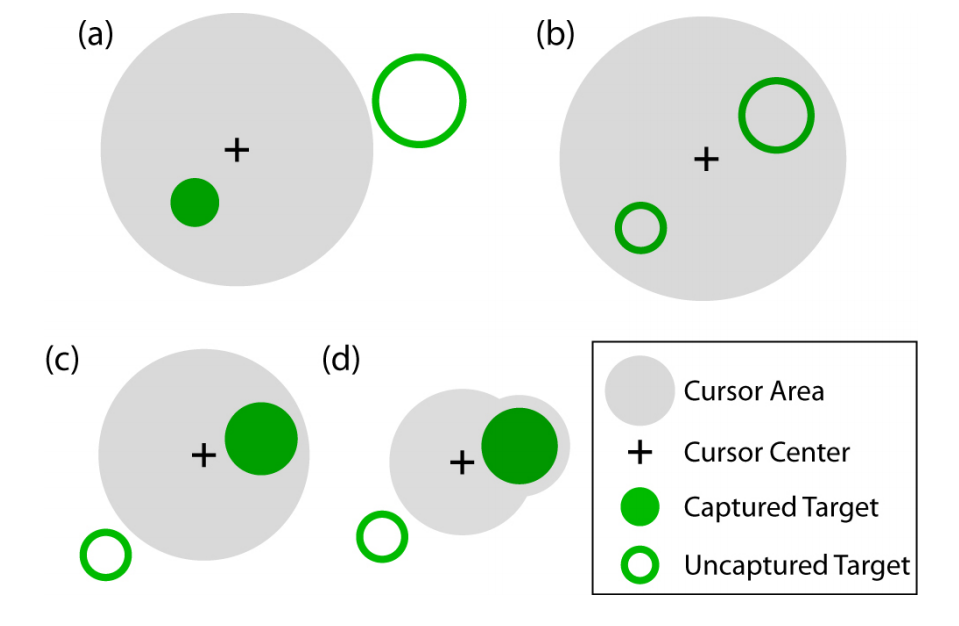
\includegraphics[width=\textwidth]{figures/bubble}
		\caption{Illustration du fonctionnement de la technique \emph{Bubble Cursor} (a, c, d) par opposition à un curseur zonal (b). Dans le cas b, le curseur zonal ne permet pas aisément de choisir aisément entre les deux cibles qui se trouvent dans la zone de sélection. Mais le \emph{Bubble Cursor} s'adapte (c et d). Crédit : Grossman \emph{et al.}}
		\label{fig:bubble}
	\end{figure}
	
	\begin{figure}[ht]
		\centering
		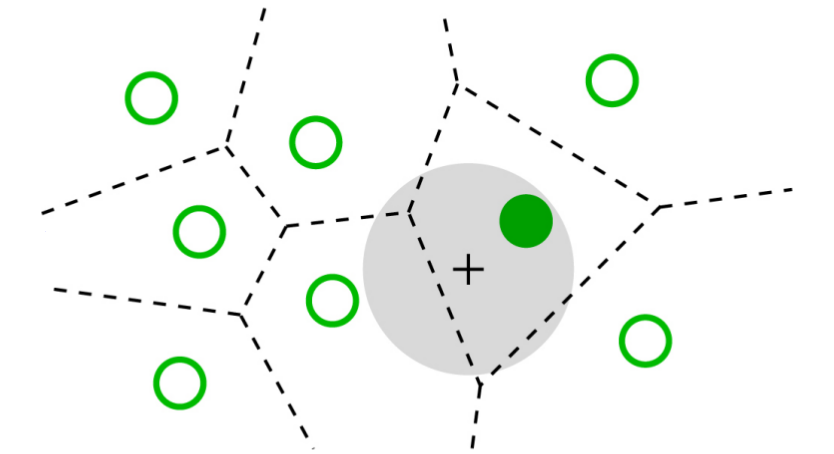
\includegraphics[width=\textwidth]{figures/voronoi}
		\caption{Diagramme de Voronoï définissant les cellules associées à chaque cible. Les frontières d'activation de chaque cible, donc sa largeur effective, sont définies par sa cellule. Crédit : Grossman \emph{et al.}}
		\label{fig:voronoi}
	\end{figure}

	\begin{figure}[ht]
		\centering
		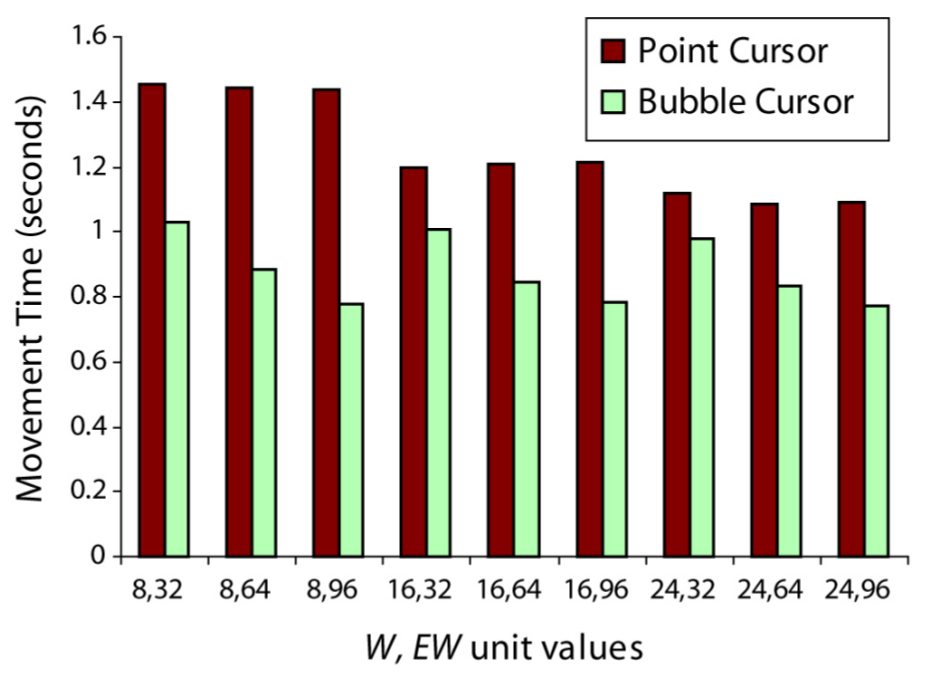
\includegraphics[width=\textwidth]{figures/bubbleResults}
		\caption{Temps mesuré pour atteindre la cible avec et sans le \emph{Bubble Cursor}, en fonction de $W$ et $EW$, où $W$ représente la largeur réelle de la cible, et $EW$ sa largeur effective, c'est-à-dire la taille de sa cellule de Voronoï. On constate que le \emph{Bubble Cursor} améliore les performances, et qu'il dépend de la largeur effective des cibles bien plus que de leur largeur réelle. Crédit : Grossman \emph{et al.}}
		\label{fig:bubbleResults}
	\end{figure}

	\subsection{Inconvénients}
	Un inconvénient de cette technique est le fait que le curseur peut rapidement croître et décroître à mesure qu'il s'approche et s'éloigne de plusieurs cibles successives. Cela peut représenter une source de distraction visuelle, en particulier quand les cibles elles-mêmes sont mobiles, \emph{a fortiori} si elles sont rapides. De plus, attendu que le \emph{Bubble Cursor} agrandit la largeur effective des cibles à la mesure de leur cellule de Voronoï, il est moins efficace en environnement dense, où les cellules de Voronoï sont plus petites. Le \emph{Bubble Cursor} montre donc ses limites face à des cibles potentielles nombreuses, mobiles et rapides.

\section{\emph{DynaSpot}}
	\subsection{Principe}
	\emph{DynaSpot} est une technique qui relie l'aire du curseur à sa vitesse. Le curseur conserve sa taille normale lorsqu'il est lent, mais croît et affecte une plus grande surface quand il de déplace plus vite. De fait il suffit de ralentir pour ramener le curseur à un comportement « normal » et pouvoir sélectionner de l'espace vide, par exemple pour ouvrir un menu contextuel, ou agir directement sur l'espace vide, comme l'illustre la figure~\ref{fig:dynaSpot}. Il n'est donc pas nécessaire de désactiver \emph{DynaSpot} ou de changer de mode explicitement. En ceci, \emph{DynaSpot} comble une des lacunes du \emph{Bubble Cursor}. Chapuis \emph{et al.}~\cite{chapuis2009dynaspot} ont montré que dans la plupart des cas, les performances de \emph{DynaSpot} sont similaires à celles du \emph{Bubble Cursor}. Ces résultats sont résumés dans la figure~\ref{fig:dynaResults}. Attendu que la croissance et la décroissance du curseur sont à la fois lentes et prévisibles avec cette technique, le niveau de distraction visuelle est faible. Par ailleurs, il n'est pas nécessaire de connaître la position des cibles potentielles pour appliquer \emph{DynaSpot}, qui ne dépend que de la vitesse du curseur.

	\begin{figure}[ht]
		\centering
		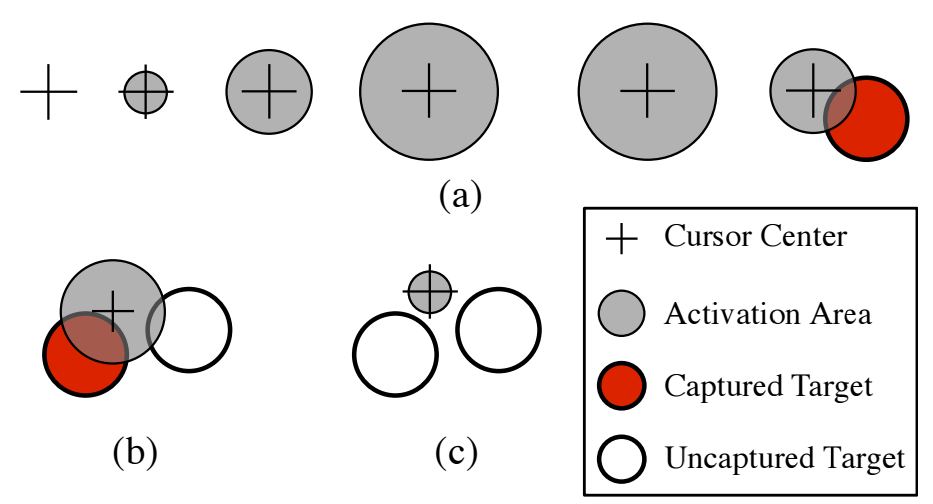
\includegraphics[width=\textwidth]{figures/dynaSpot}
		\caption{(a) La zone d'activation de \emph{DynaSpot} est couplée à la vitesse du curseur. (b) Plusieurs objets coupent la zone de sélection : la cible la plus proche du curseur est en surbrillance et sélectionnée. (c) Quand la zone de sélection ne touche aucun objet, il est possible de sélectionner l'espace vide. Crédit : Chapuis \emph{et al.}}
		\label{fig:dynaSpot}
	\end{figure}
	
	\begin{figure}[ht]
		\centering
		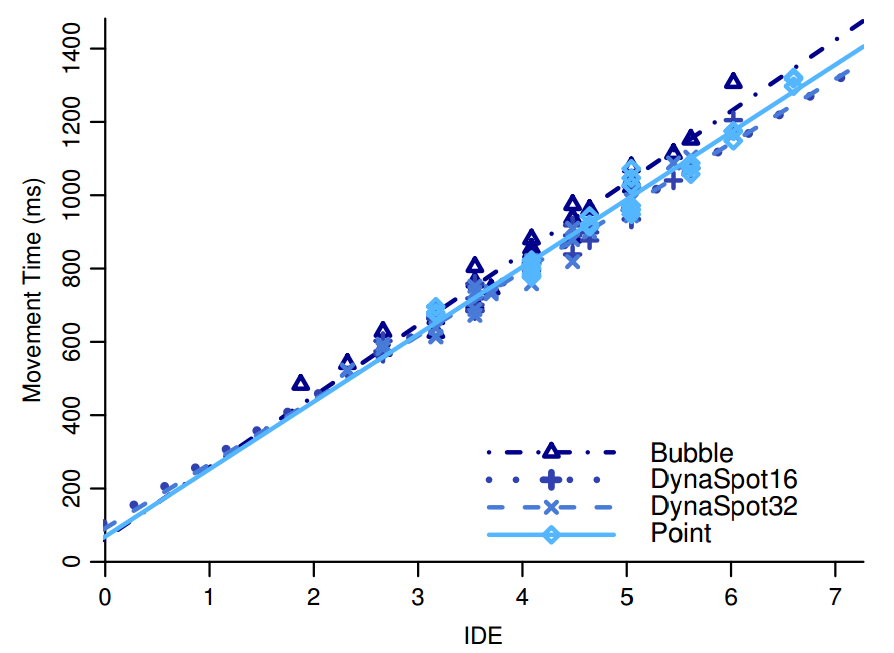
\includegraphics[width=\textwidth]{figures/dynaResults}
		\caption{Les performances (en temps de sélection) du \emph{BubbleCursor}, de \emph{DynaSpot} (dans deux versions paramétrées différemment) et d'un curseur ordinaire, en fonction de l'indice de difficulté. Celui-ci est calculé en fonction de la largeur de la cible pour le curseur ordinaire, mais en fonction de la largeur effective pour le \emph{Bubble Cursor} et \emph{DynaSpot}. Crédit : Chapuis \emph{et al.}}
		\label{fig:dynaResults}
	\end{figure}

	\subsection{Inconvénients}
	Le principal inconvénient de cette technique est précisément le fait que le curseur ne tient pas compte des cibles. Par conséquent, à vitesse élevée, sa surface peut en recouvrir plusieurs, et il ne peut déterminer laquelle est la bonne. Il est donc nécessaire de ralentir et d'attendre que le curseur rapetisse suffisamment pour ne toucher qu'une cible. En pratique, cela se produit assez rapidement, et pour les cibles statiques ce n'est pas vraiment gênant. Mais si les cibles sont mobiles, et \emph{a fortiori} rapides, le curseur ne peut s'arrêter, et il peut même être impossible à l'utilisateur de ralentir suffisamment pour que le curseur retrouve une taille permettant la sélection. Ainsi, de même que pour le \emph{Bubble Cursor}, la densité et la vitesse des cibles posent de sérieux problèmes.

	\paragraph{}	
	On pourrait toutefois envisager une sélection en deux temps : l'utilisateur pré-sélectionnerait plusieurs cibles lorsque le curseur est gros et rapide, puis devrait choisir parmi les cibles touchées laquelle il veut. Naturellement, le processus de sélection en deviendrait plus lourd et plus long.

\section{\emph{(Bubble) Comet}}
	\subsection{Principe et avantages}
	Avec \emph{Comet}, chaque cible potentielle laisse derrière elle une traînée (ou queue) qui peut être sélectionnée à la place de la cible elle-même. Cela revient à augmenter la taille effective des cibles. Attendu que cela s'applique aux cibles et pas aux curseurs, \emph{Comet} peut être combinée à une technique de curseur, par exemple le \emph{Bubble Cursor} ou \emph{DynaSpot}. \emph{Hasan et al.} ont montré que cette technique permet de significativement améliorer les temps de sélection et les taux d'erreur pour les cibles mobiles en 2D~\cite{hasan2011comet}.
	
	\begin{figure}[ht]
		\centering
		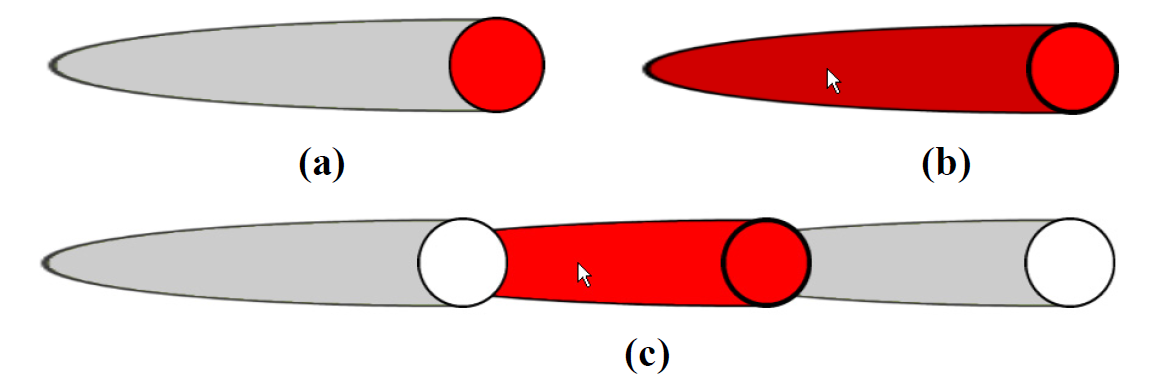
\includegraphics[width=\textwidth]{figures/comet}
		\caption{(a) La cible et sa queue de comète. (b) La queue est mise en surbrillance lorsque le curseur passe dessus. (c) Les queues peuvent être recouvertes par les cibles ajdacentes. Crédit : Hasan \emph{et al.}}
		\label{fig:comet}
	\end{figure}
	
	\begin{figure}[ht]
		\centering
		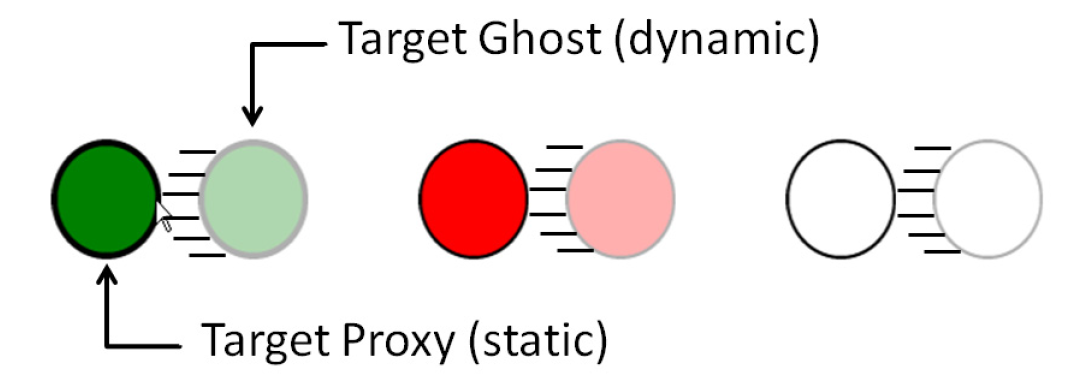
\includegraphics[width=\textwidth]{figures/targetGhost}
		\caption{(Les flèches et annotations ont été ajoutées à l'image pour l'illustrer). La technique \emph{Target Ghost} avec un curseur basique. Quand elle est « \emph{ghostée} » la cible originale voit la saturation de sa couleur baisser (en tant que fantôme) mais elle poursuit sa trajectoire. Un proxy beaucoup plus net de l'objet demeure figé à la position qu'il occupait lorsque la touche \emph{Maj} a été pressée, et il devient possible de le sélectionner. D'ailleurs, seul le proxy peut être sélectionné, pas le fantôme de la cible. Crédit : Hasan \emph{et al.}}
		\label{fig:targetGhost}
	\end{figure}
	
	\begin{figure}[ht]
		\centering
		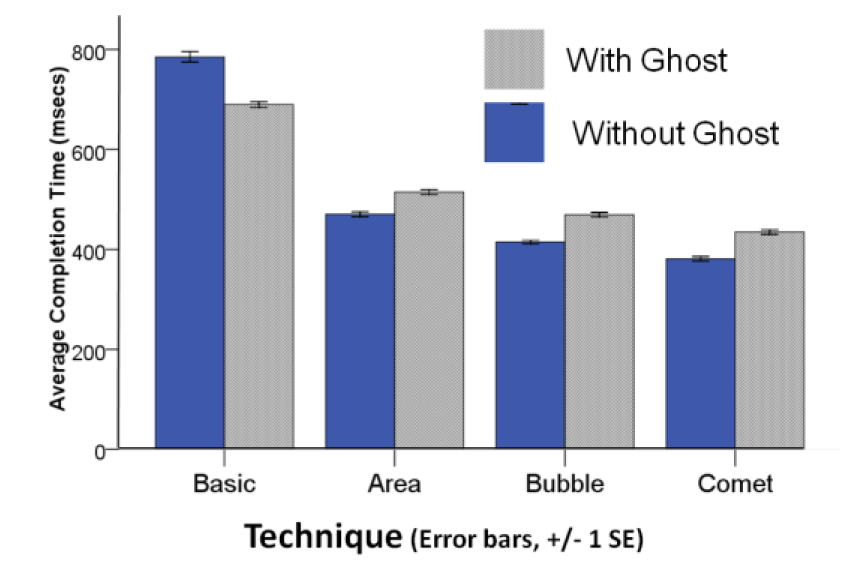
\includegraphics[width=\textwidth]{figures/cometGhostTimes}
		\caption{Temps de complétion de la tâche de sélection, avec plusieurs techniques (curseur basique, curseur zonal, \emph{Bubble Cursor} et \emph{Comet}), avec et sans \emph{Ghost}. On constate que l'usage d'un fantôme est bénéfique sur un curseur basique, mais néfaste dans tous les autres cas. Par ailleurs, \emph{Comet} offre les meilleures performances. Il ne s'agit cependant ici que du temps de sélection. Crédit : Hasan \emph{et al.}}
		\label{fig:cometGhostTimes}
	\end{figure}
	
	\begin{figure}[ht]
		\centering
		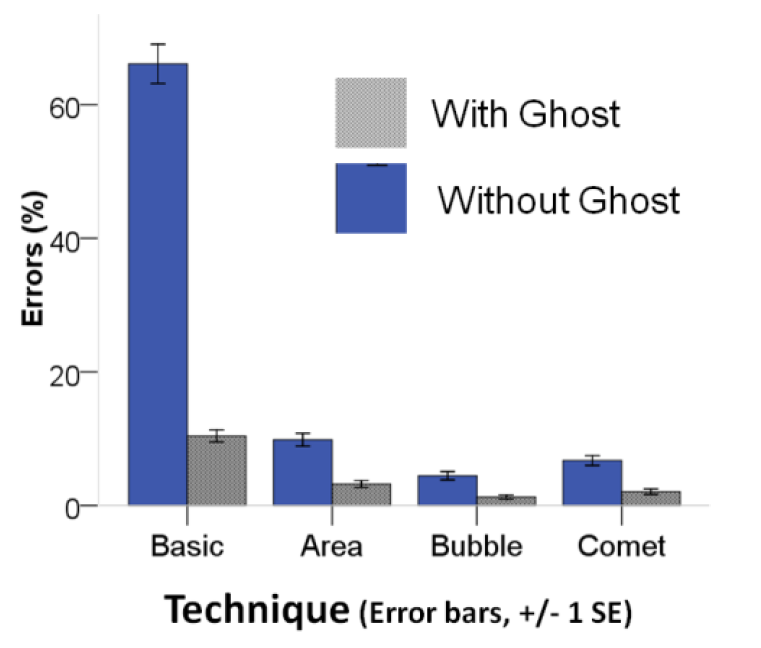
\includegraphics[width=\textwidth]{figures/cometGhostErrors}
		\caption{Taux d'erreur pour la tâche de sélection, avec plusieurs techniques (curseur basique, curseur zonal, \emph{Bubble Cursor} et \emph{Comet}), avec et sans \emph{Ghost}. On constate que l'usage d'un fantôme est très bénéfique dans tous les cas, même s'il augmente le temps de sélection lorsqu'une meilleure technique que le curseur basique est utilisée. Crédit : Hasan \emph{et al.}}
		\label{fig:cometGhostErrors}
	\end{figure}
	
	\begin{figure}[ht]
		\centering
		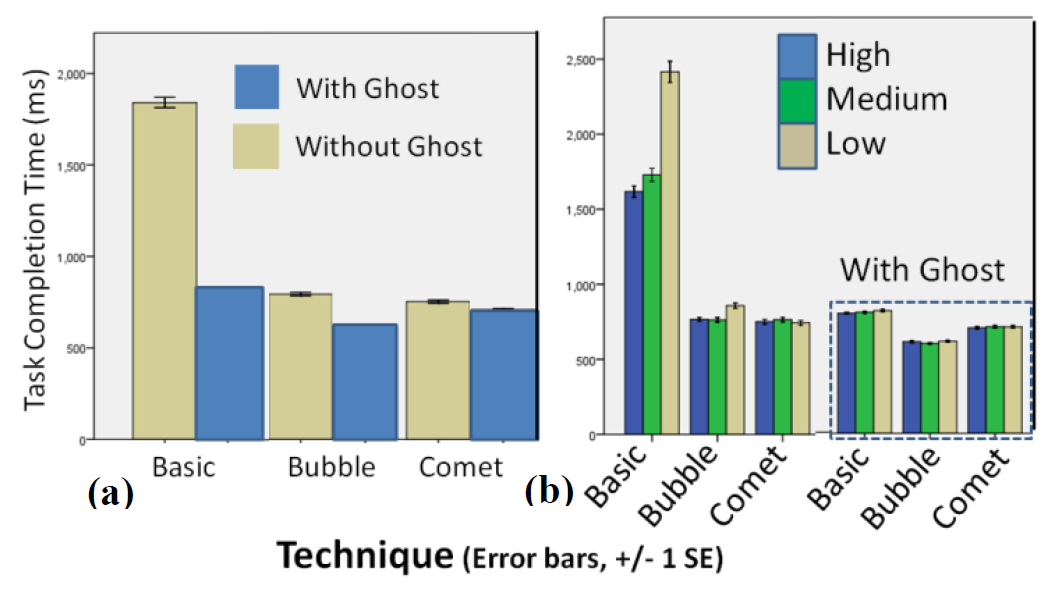
\includegraphics[width=\textwidth]{figures/cometGhostPredictability}
		\caption{Blabla. Crédit : Hasan \emph{et al.}}
		\label{fig:cometGhostPredictability}
	\end{figure}

	\subsection{Inconvénients}
	Cependant, \emph{Comet} ajoute un « encombrement » visuel important. En effet, à chaque cible vient s'ajouter une queue qui fait plusieurs fois sa taille. Étendue à la 3D, cette technique ferait logiquement usage de rendu volumique semi-transparent pour les queues de comètes, ce qui aurait probablement pour effet de porter l'encombrement visuel et donc l'occultation à des niveaux inacceptables, surtout dans des environnements denses. Un autre inconvénient de cette technique est qu'elle modifie la représentation visuelle des cibles, et en particulier de leur forme. Pour certaines applications, par exemple les simulations moléculaires (dans lequelles la perception des formes des molécules est absolument critique) ce point est particulièrement gênant. Par conséquent, la technique \emph{Comet} ne peut être retenue pour les environnements tridimensionnels denses.

\section{\emph{Target/Bubble Ghost}}
	\subsection{Principe et avantages}
	\emph{Target Ghost}[ref] est une technique qui repose sur un déclenchement délibéré. Quand elle est déclenchée par l'utilisateur, \emph{Target Ghost} duplique toutes les cibles potentielles. Une des copies est devient statique et reste opaque, tandis que l'autre demeure mobile mais est rendue semi-transparente. L'utilisateur peut ensuite sélectionner la version statique et opaque de la cible, qui sert de proxy pour sa jumelle mobile. Cela permet de ramener une tâche de sélection de cible mobile à une simple sélection de cible statique. Naturellement, cela facilite considérablement les choses, ce qui permet d'améliorer significativement les temps de sélection et, dans une plus grande mesure encore, les taux d'erreur. De plus, cette technique n'affectant que les cibles, elle peut être combinée à une technique de curseur, ce qui fut d'ailleurs fait avec le \emph{Bubble Cursor}, pour une combinaison baptisée \emph{Bubble Ghost}~\cite{hasan2011comet}.
		
	\subsection{Inconvénients}
	Là encore, l'inconvénient principal de cette technique est l'augmentation de l'encombrement visuel, puisque le nombre de cibles affichées double, même si la moitié d'entre elles sont semi-transparentes. Elle peut par ailleurs aggraver le problème d'occultation : en effet, si une cible mobile passe derrière un objet statique ou une autre cible potentielle, déclencher \emph{Target/Bubble Ghost} à cet instant aurait pour effet de prolonger indéfiniment l'occultation de cette cible. Ce problème est d'autant plus gênant que la densité de cibles potentielles est élevée.
		
	\paragraph{}
	L'utilisation d'un proxy peut aussi être gênante dans un contexte immersif avec un périphérique de saisie permettant une correspondance à l'échelle $1$ entre l'espace moteur et l'espace virtuel, en particulier si la sélection a pour but de permettre une manipulation de l'objet saisi. C'est notamment le cas pour les simulations de dynamiques moléculaires, qui impliquent d'envoyer des forces au système simulé, avec un retour (pseudo-)haptique pour l'utilisateur.
		

\section{Sélection en cascade, grossière, puis fine}
	 \subsection{Principe et avantages}
	 Les techniques de cette catégorie divisent la sélection en deux phases. Premièrement, une portion de l'espace visuel est sélectionnée. Cette première phase étant grossière, elle n'a pas besoin d'être précise, et peut être très rapide. Par exemple, avec un simple périphérique de pointage, tel qu'une souris, un ratio contrôle/affichage (\emph{control/display, C/D}) très faible pourrait être utilisé. Le curseur pourrait ainsi se placer très rapidement sur la zone d'intérêt, mais n'aurait pas besoin d'être précisément sur la cible pour délencher la deuxième phase : la sélection fine. Dans celle-ci, l'utilisateur sélectionne la cible elle-même, par exemple à l'aide d'un ratio C/D plus élevé. Du point de vue de la loi de Fitts, au cours de la phase grossière, la cible bénéficie d'une largeur accrue (car c'est toute une zone autour de la cible qui est visée) tandis que la phase fine offre une distance réduite, puisque le curseur se trouve déjà près de la cible. Quoiqu'il y ait généralement un certain « coût cognitif » lié au basculement d'une phase à l'autre, les techniques de sélection en cascade peuvent améliorer significativement les performances de sélection, même pour les tâches dont l'indice de difficulté est élevé.[mettre une bonne ref !]
		 
	\subsection{Inconvénients}
	Les techniques de sélection en cascade pouvant prendre des formes très diverses, leurs avantages et inconvénients sont également divers. Néanmoins, elles ont pour principe commun de travailler successivement à différentes échelles, ce qui pourrait être perturbant en environnement immersif, particulièrement lorsque l'on cherche à maintenir une correspondance entre l'espace moteur et l'espace virtuel. Néanmoins, si les gains de performances offerts par la sélection en cascade sont importants, cette perturbation pourrait être une contrepartie acceptable. Notons que la phase grossière ne se fait pas nécessairement avec le même périphérique que la phase fine ; elle peut par exemple se baser sur une estimation de la direction du regard de l'utilisateur, voire se faire automatiquement, par exemple lorsque l'utilisateur focalise son regard sur une zone approximativement constante pendant un certain laps de temps.


% 40% to 70% of gaze displacement is provided by head rotation, while the remaining 60% to 30% result from angular displacement of the eyes in orbit
% http://books.google.fr/books?id=h9FEnj3C7MoC&pg=PA102&lpg=PA102&dq=head+tracking+70%25+of+gaze&source=bl&ots=cp8OJm_G-1&sig=0jsxP3V20VGuxmIvg9CB1sUcyeU&hl=en&sa=X&ei=JFUsU-rVJYam0AW1zYDwAw&redir_esc=y#v=onepage&q&f=false
\section{Suivi de la tête et des yeux}
	\paragraph{}
	Une estimation de la direction du regard de l'utilisateur peut être utilisée soit pour sélectionner directement la cible (ce qui peut nécessiter beaucoup de précision, quand la cible est petite) soit pour sélectionner une zone d'intérêt, dans la phase grossière d'une sélection en cascade. Il y a au moins deux façons d'estimer la direction du regard : la première consiste à capturer les mouvements de la tête de l'utilisateur, et à supposer qu'il regarde droit devant lui. Comme cette hypothèse est généralement fausse, on génère un cone dont le sommet est la tête de l'utilisateur, et dont l'axe de révolution correspond à la direction (estimée) du regard. Or, 40~\%{} à 70~\%{} du déplacement du regard est déterminé par la rotation de la tête, tandis que le reste résulte des mouvements oculaires.[ref bouquin] Si cela s'avère souvent insuffisant pour effectuer une sélection directe, le suivi de tête peut présenter un certain intérêt pour la sélection en cascade.
		
	\paragraph{}
	Pour estimer la direction du regard avec plus de précision, on peut capturer non seulement la position et l'orientation de la tête, mais également l'orientation des yeux. Cette option séduisante présente toutefois quelques difficultés :
	\begin{itemize}
		\item Les performances dépendent de la couleur des yeux ;[ref]
		\item Le suivi des yeux ne fonctionne pas toujours bien en environnement sombre, par exemple dans un CAVE ;[ref]
		\item Les lunettes stéréoscopiques occultent partiellement les yeux pour les \emph{trackers} oculaires, et réduisent la luminosité du blanc des yeux ;[ref]
		\item Le suivi des yeux, souvent combiné à celui de la tête, est plus coûteux que celui de la tête seule ;
		\item Le fait d'utiliser ses yeux pour sélectionner un objet fait du regard une action, rend les utilisateurs conscients de la direction dans laquelle ils regardent, ce qui peut être troublant.
	\end{itemize}

	Par conséquent, l'utilisation de suivi des yeux se montre souvent difficile à mettre en œuvre, quoique les progrès techniques puissent, dans un futur proche, pallier au moins partiellement ces difficultés.
		
\section{\emph{Speed}}
	\subsection{Principe et avantages}
	\emph{Speed} est une heuristique de prédiction de cible. Quand l'utilisateur tente de sélectionner une cible, il déplace son curseur vers elle d'une façon que l'on peut séparer en deux phases. Au cours de la première phase, il accélère, tandis qu'il décélère pendant la seconde. C'est dans cette dernière que l'utilisateur est généralement le plus précis. \emph{Speed} base donc sa prédiction de cible sur la phase de décélération. L'heuristique estime la distance que le curseur finira par couvrir à partir de la vitesse du curseur, par ajustement de courbe avec celle d'une fonction quadratique. Quand le curseur a parcouru 85~\%{} de la distance totale estimée, \emph{Speed} utilise la position et la direction courantes du curseur, ainsi que l'estimation de la distance qu'il lui reste à parcourir pour prédire sa destination finale, et par conséquent, la cible visée par l'utilisateur. Cette technique fournit de meilleurs résultats que les précédentes approches de ce type qui ne faisaient pas de distinction entre les phase d'accélération et de décélération.[ref]
			
	\subsection{Inconvénients}
	Cependant, \emph{Speed} part du principe qu'au moment où l'utilisateur décide de sélectionner une cible et commence à déplacer le curseur, il sait quelle cible il veut choisir, où elle se trouve, et donc où placer son curseur. De fait, le mouvement effectué est approximativement rectiligne. Mais si les cibles sont mobiles, alors la trajectoire du curseur ne peut plus être supposée rectiligne. Par conséquent, la précision de \emph{Speed} avec des cibles mobiles est sujette à caution. C'est d'autant plus vrai en environnement dense, car une petite erreur de prédiction a d'autant plus de chances d'aboutir à la sélection d'un distracteur que ceux-ci sont nombreux et près de la cible visée.
		
\section{Hook}
	\paragraph{}
	\emph{Hook} est une heuristique de prédiction de cible. Elle se base sur une évaluation continue de la distance entre le curseur et les cibles potentielles. Celles-ci sont triées par ordre de proximité, et les $NCT$ (\emph{Number of Closest Targets} cibles les plus proches du curseur voient leur score augmenter à chaque boucle de l'heuristique, et augmenter d'autant plus fortement qu'elles sont proches du curseur. Toutes les autres cibles voient leur score diminuer, et diminuer d'autant plus fortement qu'elles sont éloignées du curseur.
		
	\paragraph{}
	La cible potentielle dont le score est le plus élevé est considérée comme celle que l'utilisateur cherche probablement à sélectionner. La sélection peut donc se faire par simple pression d'un bouton, sans contrainte particulière sur la position du curseur au moment où elle est déclenchée.
		
	\paragraph{}
	\emph{Hook} présente plusieurs avantages. Cette technique spécifiquement conçue pour les cibles mobiles fonctionne également pour les cibles statiques. Elle n'ajoute aucun encombrement visuel, ne transforme pas le curseur, ne modifie pas l'apparence des cibles, et n'interrompt pas l'animation ou la simulation en cours. L'évaluation menée par Michael Ortega montre que \emph{Hook} est non seulement plus rapide que le \emph{Bubble Cursor} en 2D comme en 3D, mais permet en plus des taux d'erreur plus faibles. Lorsque les cibles sont rapides, le taux d'erreur peut être moindre d'un facteur supérieur à 4. [ref]

\clearpage
